\PassOptionsToPackage{hyphens}{url}
\documentclass[11pt]{article}
\usepackage[T1]{fontenc}
\usepackage{lmodern}
\usepackage[margin=1in]{geometry}
\usepackage{amsmath,amssymb,amsthm,mathtools}
\usepackage{microtype}
\usepackage{booktabs}
\usepackage{enumitem}
\usepackage{float}
\usepackage[numbers,square,sort&compress]{natbib}
\usepackage{tikz}
\usetikzlibrary{arrows.meta,positioning,fit,calc,backgrounds}
\usepackage[colorlinks=true,linkcolor=blue!45!black,citecolor=blue!45!black,urlcolor=blue!45!black]{hyperref}
\hypersetup{pdftitle={Parity lifts and bounded-treewidth witnesses for Weisfeiler--Leman equivalence},pdfauthor={OpenAI}}
\newtheorem{theorem}{Theorem}[section]
\newtheorem{lemma}[theorem]{Lemma}
\newtheorem{proposition}[theorem]{Proposition}
\newtheorem{corollary}[theorem]{Corollary}
\theoremstyle{definition}
\newtheorem{definition}[theorem]{Definition}
\theoremstyle{remark}
\newtheorem{remark}[theorem]{Remark}
\numberwithin{equation}{section}
\newcommand{\FF}{\mathbb F_2}
\newcommand{\NN}{\mathbb N}
\newcommand{\RR}{\mathbb R}
\newcommand{\ind}[1]{\mathbf 1_{\{#1\}}}
\title{Parity lifts and bounded-treewidth witnesses for Weisfeiler--Leman equivalence}
\author{OpenAI}
\date{September 25, 2026}
\begin{document}
\maketitle
\begin{abstract}
For \(k\ge4\), we construct two uncolored graphs that are
\(k\)-dimensional Weisfeiler--Leman equivalent exactly when a prescribed
finite-domain choice system has no compatible choice. The system has
\(k+1\) domains for joint refinement and \(k\) for separate-coordinate
refinement. A successful choice is detected after two joint rounds or
one separate round.
Applied to sparse satisfiability, the reduction gives fixed-dimension
\(n^{\Omega(k)}\) time exclusions under positive-rate ETH, even for
deciding equality of these early histograms.
\end{abstract}

\section{Introduction}\label{sec:introduction}

The Weisfeiler--Leman method compares graphs by repeatedly refining
colors of vertex tuples. Its dimension controls how much of a graph
each tuple can describe. A useful way to study this refinement is to
count graph homomorphisms from graphs of bounded treewidth: those
counts connect local information in a tree decomposition to the global
color distribution of the target graph.

We give an explicit reduction from compatible choices in finite domains
to Weisfeiler--Leman equivalence. Its main ingredients are two parity
lifts of one base graph and a procedure that extracts compatible choices
from any distinguishing homomorphism test with sufficiently small bags.
All output graphs are finite, simple, undirected and uncolored.
The construction is independent of the computational applications in
the last section.

\subsection{Refinement and simultaneous choices}

Fix an integer \(k\ge4\). Initially, an ordered tuple
\(\mathbf x\in V(X)^k\) has its \emph{atomic type} as color: the
equalities and adjacencies between all positions. Write
\(\mathbf x[i\leftarrow y]\) for replacement of coordinate \(i\) by \(y\).
In \emph{joint} refinement, also called the correlated replacement-vector
convention, a round records the old color \(C_r(\mathbf x)\) and
\[
 \{\!\{\,\bigl(C_r(\mathbf x[1\leftarrow y]),\ldots,
                  C_r(\mathbf x[k\leftarrow y])\bigr):
                       y\in V(X)\,\}\!\}.
\]
In \emph{separate} refinement it records the old color and the \(k\)
multisets
\(\{\!\{C_r(\mathbf x[i\leftarrow y]):y\in V(X)\}\!\}\), one for
each coordinate \(i\). Colors are these data, with common names across
graphs. Two graphs are \(k\)-WL equivalent when their tuple-color
histograms agree at every round. Because each round retains the old
color, it suffices to compare until the common color partition on the
two tuple sets stabilizes.
We also consider refinement of all tuples in a disjoint union
\(X_0\sqcup X_1\), comparing the histograms on its two pure tuple sets
\(V(X_0)^k\) and \(V(X_1)^k\).

The parameter used throughout the construction is
\begin{equation}\label{eq:bag-parameter}
 t=\begin{cases}
      k+1,&\text{joint refinement},\\
      k,&\text{separate refinement}.
    \end{cases}
\end{equation}

\begin{definition}[Simultaneous choices]\label{def:choice}
A \emph{choice system} consists of finite domains \(D_1,\ldots,D_t\)
and, for every \(i<j\), a finite label set \(L_{ij}\) and maps
\[
 \lambda_{ij}^i:D_i\longrightarrow L_{ij},
 \qquad
 \lambda_{ij}^j:D_j\longrightarrow L_{ij}.
\]
A \emph{successful choice} is a tuple
\((d_1,\ldots,d_t)\in\prod_iD_i\) satisfying
\(\lambda_{ij}^i(d_i)=\lambda_{ij}^j(d_j)\) for every \(i<j\).
Empty domains are allowed.
\end{definition}

For example, let \(D_i\) be a set of Boolean assignments on a finite
variable scope \(V_i\), and let both pair maps record restriction to
\(V_i\cap V_j\), with label set \(\{0,1\}^{V_i\cap V_j}\).
A successful choice is then a family of allowed partial assignments
that joins to one assignment on \(\bigcup_i V_i\).

Thus each pair of chosen elements must give the same answer to its
shared label test. The labels are input data for the construction;
they will not become vertex colors in the output. Write
\(X_0\equiv_k X_\star\) for equivalence under the chosen convention.

\begin{theorem}[Parity reduction]\label{thm:choice-reduction}
Fix \(k\ge4\), either refinement convention, and the corresponding
\(t\) in \eqref{eq:bag-parameter}. From every choice system on \(t\)
domains one can explicitly construct two uncolored simple graphs
\(X_0,X_\star\) of equal order such that
\[
 X_0\equiv_k X_\star
 \quad\Longleftrightarrow\quad
 \text{the choice system has no successful choice}.
\]
The assertion holds both with common color names on separate graphs
and with pure-tuple comparison in their disjoint union.

If every domain and label set has size at most \(A\), where \(A\ge1\),
their common order is at most \(A M_t\), where
\[
 M_t=t\,2^{\,t-2+3\binom{t-1}{2}}+12\binom t3.
\]
When a successful choice exists, the two graphs already have different
histograms after at most two joint rounds, or one separate round.
\end{theorem}

The order bound is a bound on the actual uncolored graphs; no promise
about distinguished fibers or preserved types is supplied to a decider.

\subsection{Context and the main ideas}

Weisfeiler and Leman introduced the refinement method in their study
of graph canonization~\citep{WL1968}. The parity examples of
Cai, F\"urer and Immerman~\citep{CFI1992} are pairs of nonisomorphic
vertex-colored graphs of maximum degree three that require WL dimension
linear in their order to distinguish. The present construction also compares
parity constraints, but its purpose is to make a successful selection
from prescribed finite domains exactly equivalent to a detectable
homomorphism-count difference.

Encoding local solutions of binary linear systems as graph vertices
also underlies the construction of Atserias, Man\v{c}inska, Roberson,
\v{S}\'amal, Severini and Varvitsiotis
\citep[author version, Section~6.2]{AMRSSV2019}.
Their graphs join assignments that disagree on shared variables and
compare a system with the system obtained by setting all right-hand
sides to zero. Roberson's parity graphs instead use agreement along
adjacent constraint types.

The lift-counting argument has a close predecessor in Roberson's parity
graphs and oddomorphisms~\citep[preprint version, Definition~3.1,
Theorem~3.6 and Lemma~3.8]{Roberson2026}. We use a typed-template adaptation of that
construction: a lift retains both a base-graph vertex and the parity
tag of its template type. The comparison of homogeneous and affine
solution sets, and its dual parity certificate, follow the same
framework. We prove these facts locally in the form needed for arbitrary
projections into our base graph. The additional work is to encode pair
labels by helpers and extract a successful choice from every
bounded-bag obstruction.

Dvo\v{r}\'ak~\citep{Dvorak2010} and Dell, Grohe and
Rattan~\citep{DGR2018} connect Weisfeiler--Leman refinement with
homomorphism counts from graphs of bounded treewidth. We use their
rooted-count viewpoint and give the exact two interfaces needed here:
equality of all counts with bags of size at most \(t\) implies
\(k\)-WL equivalence, and one explicit template is detected in the
number of rounds stated in Theorem~\ref{thm:choice-reduction}.
The proof keeps the difference between \(t=k+1\) and \(t=k\) visible,
including when refinement is run on the whole disjoint union.

A graph homomorphism is a vertex map preserving adjacency; write
\(\hom(F,X)\) for the number of maps from \(F\) to \(X\).
Our template has \(t\) main vertices forming a clique. For each pair
\(i<j\) and each third main vertex \(\ell\), it has a helper adjacent
to \(i,j,\ell\). The base graph replaces main type \(i\) by its domain
\(D_i\) and this helper type by a copy of \(L_{ij}\). Main edges and the
two helper edges toward \(i,j\) enforce label agreement; the helper
edge toward \(\ell\) is unrestricted.

The parity lifts replace each base vertex by bit vectors indexed by
its neighboring template types. Each vector has a prescribed parity,
and two vectors over a base edge must agree in the coordinates facing
each other. The two lifts differ only in the parity at main type \(1\).
For a fixed projected homomorphism into the base, the lifts to \(X_0\)
form the kernel of a binary linear system. Those to \(X_\star\) form
either a translate of the kernel or the empty set. Every projection
therefore contributes a nonnegative difference to
\(\hom(F,X_0)-\hom(F,X_\star)\). A single positive contribution cannot
be cancelled by other, possibly non-type-preserving homomorphisms.

A successful choice supplies such a contribution from the template
itself. Conversely, a distinguishing test gives a dual parity
certificate consisting of weights on its vertices and edges. For a
test with bags of size at most \(t\), these weights orient each edge of
a tree decomposition toward an odd side. A sink bag contains one
representative of every main type. This odd-side orientation is closely
related to Neuen and Seppelt's separator argument for oddomorphisms
\citep[Lemma~4.4 and proof of Theorem~4.1]{NS2026}.
The remaining issue is the representatives'
compatibility: a bag need not induce a clique, and its representatives
need not have nonzero weight. The helper associated with a mismatched
pair transfers its weighted discrepancy to whichever main type is
absent from a separator. The resulting boundary identity rules out
the mismatch, even with repeated projected images and zero weights.

Section~\ref{sec:wl-tests} proves the two homomorphism interfaces.
Section~\ref{sec:parity-lifts} constructs the graphs and establishes
noncancellation and the explicit positive witness.
Section~\ref{sec:separator} proves extraction and completes
Theorem~\ref{thm:choice-reduction}.
Section~\ref{sec:complexity} applies the construction to satisfiability.

\subsection{Conditional time bounds and their scope}

For fixed \(k\), direct refinement decides equivalence in
\(n^{O(k)}\) time. The complexity question is whether this growing
exponent can be avoided by a different algorithm.

The \emph{positive exponential-rate ETH} of Impagliazzo and
Paturi~\citep{IP2001} asserts that some \(\delta>0\) rules out a
deterministic \(3\)-SAT algorithm with running time
\(2^{\delta N}\operatorname{poly}(L)\), where \(N\) is the number of
variables and \(L\) the formula encoding length. This is the hypothesis
for the following fixed-dimension application.

\begin{theorem}[Fixed-dimension ETH consequence]\label{thm:eth}
Assume positive exponential-rate ETH. There are constants \(c>0\)
and \(K\ge4\) such that, for every fixed integer \(k\ge K\), no
deterministic algorithm decides \(k\)-WL equivalence of two
\(n\)-vertex graphs in time \(O(n^{ck})\).
This holds for both joint and separate refinement. The inputs are
explicit adjacency matrices of uncolored simple undirected graphs,
and time is measured on a multitape Turing machine.
\end{theorem}

The hypothetical algorithm and its multiplicative constant may depend
arbitrarily on the fixed \(k\); the constants \(c,K\) do not.
Theorem~\ref{thm:eth} therefore excludes even an ineffectively selected
family of solvers whose running-time exponents are \(o(k)\).
Under the weaker premise excluding one
uniform \(2^{o(N)}\operatorname{poly}(L)\)-time \(3\)-SAT algorithm, we
instead prove the uniform \(f(k)n^{o(k)}\) exclusion in
Proposition~\ref{prop:uniform}. Its algorithm receives \(k\) as input.
These hypotheses are kept separate throughout the parameter analysis.

Bounds on the number of refinement rounds concern a different question.
For each fixed \(k\ge2\), Grohe, Lichter, Neuen and Schweitzer
\citep[preprint version, Theorem~1 and Corollary~34]{GLNS2025}
construct colored graph pairs requiring \(\Omega(n^{k/2})\) rounds of
joint refinement. Such a bound constrains the refinement process itself;
it does not rule out a faster algorithm deciding its stable equivalence
relation.
The time exclusions proved here already apply to comparing tuple-color
histograms after two joint rounds or one separate round, under the same
respective hypotheses; Section~\ref{sec:complexity} gives the deduction.

Lichter, Ra{\ss}mann and Schweitzer~\citep[Section~6]{LRS2025}
expressed the expectation that neither equivalence nor identification
admits \(n^{o(k)}\) time and suggested lower bounds based on ETH or
its strong form.
The application above concerns the equivalence question.
The companion article \emph{Unconditional time lower bounds for
Weisfeiler--Leman equivalence}~\citep[Theorem~1.1]{CompanionUnconditional}
proves a stronger time bound: for every sufficiently large fixed \(k\)
and every correct deterministic decider, an absolute exponent linear
in \(k\) is required at every sufficiently large graph order.
It also obtains connected graphs of diameter at most two.
Its unconditional theorem supersedes the conditional lower bound for
stable equivalence in Theorem~\ref{thm:eth}.
The contribution of this article is the explicit choice reduction
and its helper-based bounded-bag extraction, using the parity-lift and
noncancellation framework described above. No part of its proof uses
that companion theorem.

For the ETH application, the sparsification lemma of Impagliazzo,
Paturi and Zane~\citep{IPZ2001} reduces a formula to sparse disjuncts.
Partitioning their clauses into \(t\) groups gives domains of size
\(2^{O(N/t)}\): each domain consists of the assignments satisfying
one group, and pair labels are restrictions to common variables.
We retain the sparsification rate, its dependent density constant,
the explicit matrix-writing cost and the simulator's input cost in
the full calculation. Extensions to other machine models require an
absolute-power Turing simulation, as specified in
Section~\ref{sec:complexity}.

\section{WL refinement and homomorphism tests}\label{sec:wl-tests}

We use the refinement conventions and parameter \(t\) from
Section~\ref{sec:introduction}; throughout \(k\ge4\).
We will use homomorphism counts in two ways to connect the construction to WL.
Equality of all counts from sources with small bags will prove
equivalence. A difference for one explicit template will prove
inequivalence, already after two joint rounds or one separate round.

A graph has \emph{bag size at most \(t\)} if it has a tree decomposition
on a finite tree with bags of size at most \(t\): the bags containing any vertex form a
nonempty connected subtree, and some bag contains both ends of each
edge. Equivalently, its treewidth is at most \(t-1\).
Write \(\hom(F,X)\) for the number of homomorphisms from \(F\) to \(X\),
that is, vertex maps preserving adjacency.

\begin{definition}\label{def:template}
The template \(T=T_t\) has main vertices \([t]\) forming a clique.
For each \(i<j\) and \(\ell\in[t]\setminus\{i,j\}\), it has a helper
\(h_{ij;\ell}\) adjacent precisely to \(i,j,\ell\).
\end{definition}
Its main clique bag, with one attached bag
\(\{i,j,\ell,h_{ij;\ell}\}\) per helper, gives bag size at most \(t\),
since \(t\ge4\).
Every main triple supports three helpers. Consequently
\begin{equation}\label{eq:template-size}
 |V(T)|=t+3\binom t3,\qquad
 \deg_T(i)=t-1+3\binom{t-1}{2},\qquad
 \deg_T(h_{ij;\ell})=3.
\end{equation}
In particular \(T\) is connected and every vertex has positive degree.

We first establish the preservation statement for arbitrary sources
with bags of size at most \(t\), then prove the detection statement
for \(T_t\).
The homomorphism characterization of WL is established in
\citet{Dvorak2010,DGR2018}. We give a self-contained adaptation of the
rooted-count argument for the preservation direction.

\begin{lemma}\label{lem:hom-implies-wl}
If \(\hom(F,X_0)=\hom(F,X_1)\) for every graph \(F\) of bag size at most
\(t\), then \(X_0,X_1\) are \(k\)-WL equivalent in the corresponding
convention. This also holds for the disjoint-union implementation.
\end{lemma}

\begin{proof}
We realize WL updates by operations on rooted counts, then recover
color indicators on the fixed finite targets by interpolation.
Equip \(F\) with a list \(\boldsymbol\ell=(\ell_1,\ldots,\ell_k)\) of
roots, allowing repetitions, all contained in a designated bag.
Let \(h_F(X,\mathbf x)\) count homomorphisms sending \(\ell_i\) to \(x_i\),
and let \(\mathcal A_t\) be the rational span of these functions for
sources with bag size at most \(t\).
Distinct isolated roots give the constant \(1\); repeating a root tests
equality, and joining two roots tests adjacency. Complements and products
therefore give atomic-type indicators.

Here is the decomposition invariant behind the algebra.
To glue rooted graphs along an interface, attach their designated bags
to a central bag of formal interface vertices and identify each root
with its assigned interface vertex. In each operand, every merged
vertex is a root, so its occurrence subtrees meet the designated bag.
Their quotient occurrences connect through the central bag. Other
vertices retain their connected occurrence subtrees, and taking images
of bags never increases their sizes. Parallel edges may be collapsed;
a loop gives the zero function on simple targets. The central bag
contains the output roots, so this invariant persists under successive
operations. In particular, gluing corresponding roots realizes products
in \(\mathcal A_t\), with an interface of size at most \(k\).

For joint refinement, the same construction gives closure under
\[
 (f_1,\ldots,f_k)\longmapsto
 \left[(X,\mathbf x)\longmapsto
       \sum_{y\in V(X)}\prod_{i=1}^k
                      f_i(X,\mathbf x[i\leftarrow y])\right].
\]
For rooted counts, use a central bag of formal vertices
\(u_1,\ldots,u_k,y\), attach operand \(i\) at its replacement list, and
retain \(u_1,\ldots,u_k\) as output roots. This uses \(k+1=t\) vertices;
multilinearity handles their linear combinations.
Repeated roots can force \(y=u_j\) or merge old positions, precisely
enforcing the corresponding equalities in the summation.

For separate refinement only
\(f\mapsto\sum_y f(X,\mathbf x[i\leftarrow y])\) is needed.
Use adjacent bags
\(O=\{u_1,\ldots,u_k\}\) and
\(R=\{u_j:j\ne i\}\cup\{y\}\), and attach the operand's root bag to \(R\).
Each has size at most \(k=t\).
After the root identifications, a merged class meeting both \(O\)
and the operand contains a surviving \(u_j\), so it also meets \(R\).
Thus no occurrence gap is created, even when \(y=u_j\).
The old \(u_i\) remains a pinned output root in \(O\).
A homomorphism of the quotient specifies exactly one allowed image
of \(y\) and one operand homomorphism: an identification restricts that
image, rather than contributing an additional free choice.

Fix the two finite targets. At each round, every color indicator
restricted to tuples of these targets agrees with a function in
\(\mathcal A_t\). Indeed the update operations give the
multiplicity of each color vector (or each coordinate color).
If such a multiplicity \(M\) has attained values \(S\), its value-\(q\)
indicator is the polynomial
\(\prod_{s\in S\setminus\{q\}}(M-s)/(q-s)\), for \(q\in S\).
Products with the old-color indicator give every new-color indicator.
The coefficients are common to the two targets. Finally,
\(\sum_{\mathbf x\in V(X)^k}h_F(X,\mathbf x)=\hom(F,X)\):
each homomorphism specifies one root-image tuple, even with repeated
roots. The hypothesis therefore equates all color histograms.

For the union implementation, perform the indicator induction on
\emph{all} tuples of \(U=X_0\sqcup X_1\), including mixed tuples.
The interpolation coefficients are then fixed before either pure
restriction is summed. For the final quotient source \(F\), let
\(\mathcal L\) be its components containing roots and \(\mathcal R\)
its rootless components. The exact identity is
\begin{equation}\label{eq:pure-tuple-factorization}
 \sum_{\mathbf x\in V(X_j)^k}h_F(U,\mathbf x)
   =\prod_{Q\in\mathcal L}\hom(Q,X_j)
      \prod_{Q\in\mathcal R}\hom(Q,U).
\end{equation}
Connectedness forces each rooted component into \(X_j\); rootless
components are unrestricted. Every map still determines one tuple.
Different source components may share target images, so their choices
remain independent. Components inherit the bag bound, the first
product agrees for \(j=0,1\), and the second is common.
Applying this identity to each term of a color indicator proves the
claim.
\end{proof}

It remains to show that a count difference for the template \(T_t\)
is visible in the claimed number of rounds. Its helpers have only
three neighbors, so their possible images can be counted from
triple common-neighbor counts.

\begin{lemma}\label{lem:test-detected}
The round-two color histogram in joint \(k\)-WL determines
\(\hom(T_{k+1},X)\). The round-one histogram in separate \(k\)-WL
determines \(\hom(T_k,X)\). The same statements hold for pure-tuple
histograms obtained by refining a disjoint union.
\end{lemma}

\begin{proof}
Let \(A_X(v,w)=\ind{vw\in E(X)}\).
For main images \(\mathbf z=(z_1,\ldots,z_t)\), put
\(q_B(\mathbf z)=|\bigcap_{b\in B}N_X(z_b)|\), for triples \(B\subseteq[t]\).
Their number of extensions to \(T\) is
\[
 E_X(\mathbf z)=
       \prod_{a<b} A_X(z_a,z_b)
       \prod_{B\in\binom{[t]}3}q_B(\mathbf z)^3.
\]
The clique factor rejects repeated main images. Helper images may
coincide, so their choices are independent and the displayed product
is exact.

First consider joint refinement. A round-one color of a
\(k\)-tuple determines each triple common-neighbor count on its positions.
For one candidate \(w\), its atomic replacement vector reveals adjacency
to position \(p\) in any component replacing a coordinate other than \(p\).
Thus that one vector tests simultaneous adjacency to the whole triple;
summing its multiplicities gives the count.

Now fix \(\mathbf x=(z_1,\ldots,z_k)\) and set \(z_{k+1}=y\).
Its old round-one color and the single vector
\[
 \bigl(C_1(\mathbf x[1\leftarrow y]),\ldots,
       C_1(\mathbf x[k\leftarrow y])\bigr)
\]
give the round-one colors of all \(k\)-position faces of these \(k+1\)
main positions. The old tuple omits \(k+1\); replacement face \(i\)
omits \(i\), with its coordinate \(i\) representing position \(k+1\).
Every pair and triple lies in a face, since \(k\ge4\).
Reading it from, for example, the face omitting the least position
outside it determines every factor of \(E_X(\mathbf x,y)\).
All faces in this vector refer to the same \(y\).
The round-two multiset therefore determines
\(\sum_y E_X(\mathbf x,y)\); summing over tuple colors gives
\(\hom(T_{k+1},X)\).

For separate refinement, all \(t=k\) main images are already fixed.
For a triple \(B\), choose \(i\notin B\). If \(M_i(\sigma)\) is the
multiplicity of atomic type \(\sigma\) in the \(i\)-th replacement
multiset, then
\[
 q_B(\mathbf x)=\sum_\sigma M_i(\sigma)
                    \prod_{p\in B} A_\sigma(i,p),
\]
where \(A_\sigma(i,p)\) is its adjacency bit.
Thus the round-one color determines \(E_X(\mathbf x)\), and its
histogram determines \(\hom(T_k,X)\).

Finally take a pure tuple in \(X_j\) while refining \(U=X_0\sqcup X_1\).
In the joint case, a last main image outside \(X_j\) makes the
clique factor zero. Once all main images lie in \(X_j\), every common
neighbor of a triple lies there too. Hence the same formulas, evaluated
in \(U\), count precisely the desired extensions into \(X_j\).
\end{proof}

\section{Choices and parity lifts}\label{sec:parity-lifts}

Fix \(k\ge4\), and let \(t\) and \(T=T_t\) be as in
Section~\ref{sec:wl-tests}. We encode compatible choices by two uncolored
graphs. The comparison will account for every homomorphism into these
graphs, including those whose projections do not describe a choice.

Take a choice system as in Definition~\ref{def:choice}. Form a base graph \(G\) with disjoint vertex sets
\[
 \{(i,d):d\in D_i\}\quad(i\in[t]),\qquad
 \{(h_{ij;\ell},q):q\in L_{ij}\}
 \quad(i<j,\ \ell\notin\{i,j\}).
\]
The first coordinate defines a type map \(\tau:V(G)\to V(T)\).
Its edges are exactly the following, for each permitted \(i,j,\ell\):
\begin{itemize}[nosep]
\item \((i,d)\) and \((j,e)\) are adjacent if
  \(\lambda_{ij}^i(d)=\lambda_{ij}^j(e)\).
\item \((h_{ij;\ell},q)\) is adjacent to \((i,d)\) if
  \(q=\lambda_{ij}^i(d)\), and to \((j,e)\) if
  \(q=\lambda_{ij}^j(e)\).
\item Every \((h_{ij;\ell},q)\) is adjacent to every
  \((\ell,f)\), \(f\in D_\ell\).
\end{itemize}
Thus \(G\) is simple and \(\tau\) is a homomorphism to \(T\).
When evaluating a label map, we identify a vertex in a domain copy
with its underlying domain element. Types and labels are construction
data, not vertex colors supplied to WL. Figure~\ref{fig:helper-incidence}
isolates the two label tests and the unrestricted third incidence.

\begin{figure}[H]
\centering
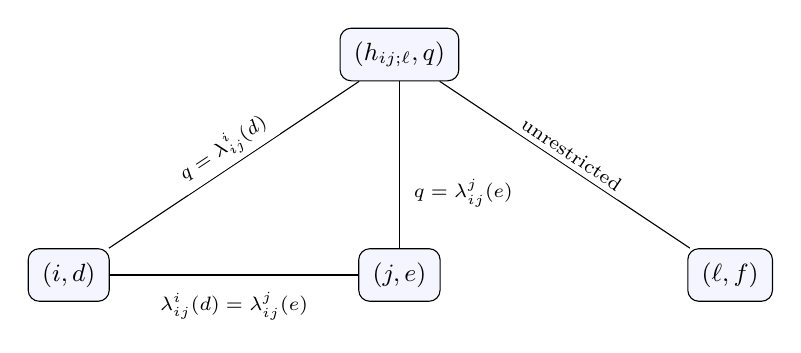
\begin{tikzpicture}[
  vertex/.style={draw,rounded corners,fill=blue!4,inner sep=5pt},
  every node/.style={font=\small},
  test/.style={font=\scriptsize,fill=white,inner sep=2pt}
]
\node[vertex] (left) at (-4.2,0) {\((i,d)\)};
\node[vertex] (middle) at (0,0) {\((j,e)\)};
\node[vertex] (right) at (4.2,0) {\((\ell,f)\)};
\node[vertex] (helper) at (0,2.8) {\((h_{ij;\ell},q)\)};
\draw (helper) -- node[test,sloped,above] {\(q=\lambda_{ij}^i(d)\)} (left);
\draw (helper) -- node[test,pos=.67,right=3pt] {\(q=\lambda_{ij}^j(e)\)} (middle);
\draw (helper) -- node[test,sloped,above] {unrestricted} (right);
\draw (left) -- node[test,below=4pt] {\(\lambda_{ij}^i(d)=\lambda_{ij}^j(e)\)} (middle);
\end{tikzpicture}

\caption{Allowed incidences for one helper in the base graph. The edges
from the helper to types \(i,j\) require its label \(q\) to equal the
corresponding pair label. Its incidence with type \(\ell\) is unrestricted.
The displayed main edge also requires pair-label agreement; other main
edges are omitted. Each labeled point denotes an arbitrary vertex of
its fiber, so an edge is present only when its indicated condition holds.}
\label{fig:helper-incidence}
\end{figure}

Write \(\FF\) for the field with two elements.
\begin{definition}[Parity lifts]\label{def:lifts}
For \(b\in\FF^{V(T)}\), the graph \(X_b\) has vertices
\[
 (u,z),\qquad
 u\in V(G),\quad z\in\FF^{N_T(\tau(u))},\quad
 \sum_{a'\in N_T(\tau(u))}z(a')=b(\tau(u)).
\]
Vertices \((u,z)\) and \((v,w)\) are adjacent precisely when
\(uv\in E(G)\) and \(z(\tau(v))=w(\tau(u))\).
We compare \(X_0\) and \(X_\star:=X_{e_1}\), where
\(e_1(a)=\ind{a=1}\).
\end{definition}

The coordinates of a tag are indexed by neighbor types in \(T\),
including types for which \(u\) has no neighbor in \(G\).
Every type has positive degree. Hence every \(u\) has
\(2^{\deg_T(\tau(u))-1}\) tags for either parity, so both output graphs
have order \(\sum_{u\in V(G)}2^{\deg_T(\tau(u))-1}\).
Both graphs are uncolored and simple: adjacency is symmetric, and a
loop would require a loop in \(G\). The map
\(\pi_b:(u,z)\mapsto u\) is a homomorphism \(X_b\to G\).
If each base fiber has at most \(A\) vertices, Equation~\ref{eq:template-size}
gives the bound \(A M_t\) of Theorem~\ref{thm:choice-reduction}:
the \(t\) main fibers have \(2^{t-2+3\binom{t-1}{2}}\) tags per base vertex,
and the \(3\binom t3\) helper fibers each have four.

The tags on the template itself form Roberson's parity graph
\citep[preprint version, Definition~3.1]{Roberson2026}. Here we additionally remember a
vertex \(u\in G\) whose type matches the tag. Equivalently, if
\(R_b(T)\to T\) is that parity graph's type projection, then \(X_b\)
is the graph on pairs in \(G\times R_b(T)\) with matching projections,
with adjacency in both coordinates. Thus fixing \(\phi:F\to G\)
fixes the template projection \(\tau\phi\). The following proof gives
the resulting local form of Roberson's lift-count comparison and binary
duality~\citep[preprint version, Theorem~3.6 and Lemma~3.8]{Roberson2026}; the compatibility
extraction in Section~\ref{sec:separator} will use the particular
helper structure of our base graph.

\begin{lemma}[Lift counts and their dual obstruction]\label{lem:lift-duality}
For every finite simple graph \(F\),
\(\hom(F,X_0)\ge\hom(F,X_\star)\).
The inequality is strict if and only if there are a homomorphism
\(\phi:F\to G\), vertex weights \(s:V(F)\to\FF\), and edge weights
\(r:E(F)\to\FF\) such that, writing \(a=\tau\circ\phi\),
\begin{equation}\label{eq:dual}
 \begin{aligned}
 \sum_{\substack{y:\,xy\in E(F)\\a(y)=a'}}r(xy)
   &=s(x)
   &&\bigl(x\in V(F),\ a'\in N_T(a(x))\bigr),\\
 \sum_{\substack{x\in V(F)\\a(x)=1}}s(x)&=1.
 \end{aligned}
\end{equation}
Whenever \eqref{eq:dual} holds, the type masses satisfy
\begin{equation}\label{eq:type-mass}
 m_u(A):=\sum_{\substack{x\in A\\a(x)=u}}s(x),
 \qquad
 m_u(V(F))=1
 \quad\bigl(u\in V(T),\ A\subseteq V(F)\bigr).
\end{equation}
All sums of weights are in \(\FF\).
\end{lemma}

\begin{proof}
Fix \(\phi:F\to G\). Its lifts to \(X_b\) correspond to solutions in
variables \(z_{x,a'}\), one for each source vertex \(x\) and each
\(a'\in N_T(a(x))\), of
\[
 \sum_{a'\in N_T(a(x))}z_{x,a'}=b(a(x))
 \quad(x\in V(F)),\qquad
 z_{x,a(y)}+z_{y,a(x)}=0
 \quad(xy\in E(F)).
\]
Indeed a solution gives the map \(x\mapsto(\phi(x),z_x)\), and a lift
uniquely determines these source-indexed vectors.
Equality of projected images does not itself identify these
source-indexed tag variables; all constraints on them are given by
the displayed system.

The coefficient matrix is independent of \(b\). The system for \(b=0\)
has its kernel as solution set; for \(b=e_1\) the solution set is
either empty or a translate of that kernel. Every homomorphism into
\(X_b\) has a unique projection to \(G\), so summing over all \(\phi\)
proves the inequality. Since each homogeneous system is nonempty,
strictness is equivalent to inconsistency of at least one projected
system for \(X_\star\). In particular, contributions from other
projections cannot cancel a strict inequality.

A binary system \(Mz=c\) is inconsistent exactly when some linear
combination of its rows has left side zero and right side one.
For the nontrivial direction, if \(c\notin\operatorname{im}M\), extend
a basis of \(\operatorname{im}M\) by \(c\) to obtain a linear functional
vanishing on \(\operatorname{im}M\) and taking value one at \(c\).
Let \(s(x)\) and \(r(xy)\) be the coefficients of the vertex and edge
equations above. The coefficient of \(z_{x,a'}\) in their combination is
\(s(x)+\sum_{y:\,xy\in E(F),\,a(y)=a'}r(xy)\),
and the right side for \(X_\star\) is \(\sum_{a(x)=1}s(x)\).
This gives exactly \eqref{eq:dual}, without any independence assumption
on the equation rows.

For adjacent types \(u,v\), sum the first equation of
\eqref{eq:dual} over all vertices of type \(u\), using neighbor type
\(v\). The result is the total \(r\)-weight of the edges between these
two types. Summing from type \(v\) gives the same total, so
\(m_u(V(F))=m_v(V(F))\). Since \(T\) is connected and
\(m_1(V(F))=1\), every type mass is one.
\end{proof}

\begin{lemma}[A choice supplies a witness]\label{lem:choice-witness}
A successful choice gives
\(\hom(T,X_0)>\hom(T,X_\star)\), and hence \(X_0,X_\star\)
are not \(k\)-WL equivalent.
\end{lemma}

\begin{proof}
Given a successful choice \((d_i)_{i\in[t]}\), map main vertex \(i\)
to \((i,d_i)\) and each \(h_{ij;\ell}\) to
\((h_{ij;\ell},\lambda_{ij}^i(d_i))\).
The common pair label and the unrestricted edge toward \(\ell\)
make this a homomorphism \(\phi:T\to G\) with
\(\tau\circ\phi\) the identity. Set every vertex and edge weight to
one. Each vertex of \(T\) has exactly one neighbor of each adjacent
type, and exactly one source vertex has type \(1\), so
\eqref{eq:dual} holds. Apply Lemma~\ref{lem:lift-duality} and then
Lemma~\ref{lem:test-detected}.
\end{proof}


A successful choice has now supplied a noncancelling, explicitly detected
witness. It remains to prove that a small-bag witness cannot arise without
such a choice. The next section extracts one directly from the dual
weights of Lemma~\ref{lem:lift-duality}.

\section{Extracting a choice from a bounded-bag witness}
\label{sec:separator}

The dual equations force odd total weight at every type.
We now use small separators to locate one bag whose main vertices
give compatible choices.
The odd-side orientation below is closely related to the separator
argument for oddomorphisms of Neuen and Seppelt
\citep[Lemma~4.4 and proof of Theorem~4.1]{NS2026}.
Here the helper types additionally force compatibility of the
representatives; we retain the local orientation to control the
weighted contribution of every outer side.

\begin{lemma}[Choice extraction]\label{lem:extract-choice}
Let \(F\) have a tree decomposition with bags of size at most \(t\).
Suppose that a homomorphism \(\phi:F\to G\) and weights
\(s:V(F)\to\FF\) and \(r:E(F)\to\FF\) satisfy
\eqref{eq:dual}, where \(a=\tau\circ\phi\).
Then the choice system has a successful choice.
\end{lemma}

\begin{proof}
All sums in this proof are in \(\FF\).
We use the type masses \(m_u(Y)\) from \eqref{eq:type-mass};
in particular, \(m_u(V(F))=1\) for every type \(u\).

\smallskip
\noindent\emph{Orienting the decomposition.}
Fix a decomposition tree \(\mathcal D\), and contract edges joining
identical bags.  Every remaining edge has an intersection \(S\) of
size at most \(t-1\): an intersection of size \(t\) would force both
incident bags to be that same set.
Deleting the tree edge partitions \(V(F)\) into \(S\) and two sides
\(A^0,A^1\).  Indeed, the occurrence subtree of a vertex outside \(S\)
lies in just one of the two tree components.  No graph edge joins the
two sides, since its endpoints occur together in a bag.

At least one main type is absent from \(S\).
If two main types \(u,v\) are absent, all \(uv\)-edges incident with
either type on a side stay on that side.  Summing \eqref{eq:dual}
over their two endpoint classes gives
\(m_u(A^\nu)=m_v(A^\nu)\) for \(\nu\in\{0,1\}\).
For any absent main type \(u\),
\[
m_u(A^0)+m_u(A^1)=m_u(V(F))=1.
\]
Orient the tree edge toward the side of mass \(1\).
This is well defined whether there is one absent main type or several.

Choose a sink of the oriented tree and denote its bag by \(B\).
For each incident edge let \(A\) be its outer side and \(S\subseteq B\)
its intersection.  These outer sides partition \(V(F)\setminus B\).
To see this precisely, the occurrence subtree of a vertex outside
\(B\) avoids the sink node and lies in exactly one component of
\(\mathcal D\) minus that node.  A vertex in \(B\) occurring in a branch
must belong to that branch's intersection \(S\), so is excluded from
its outer side.  Thus vertices are counted once, regardless of how
many bags contain them.  Moreover, every neighbor of \(A\) outside
\(A\) lies in \(S\), and the sink orientation gives
\[
m_\ell(A)=0
\qquad\text{for every main type \(\ell\) absent from \(S\).}
\]
If a main type were absent from \(B\), it would be absent from every
such \(S\) and have mass zero in the bag and in all outer sides,
contrary to its global mass \(1\).
Since \(|B|\le t\), the bag therefore consists of exactly one vertex
\(x_i\) of each main type \(i\), and no helper vertices.
No condition on the individual weights \(s(x_i)\) is needed.

\smallskip
\noindent\emph{A global mismatch test.}
Write \(\phi(x_i)=(i,d_i)\), with \(d_i\in D_i\).
The bag \(B\) need not induce a clique, so compatibility of these
representatives does not follow from \(\phi\) alone.
Suppose, for a contradiction, that some pair \(i<j\) has different
labels, and put \(\alpha=\lambda_{ij}^i(d_i)\).
We choose label predicates that vanish on these representatives and are
complementary on matching labels. For source vertices of types \(i,j\),
respectively, put
\[
p_i(x)=\ind{\lambda_{ij}^i(\phi(x))\ne\alpha},
\qquad
p_j(x)=\ind{\lambda_{ij}^j(\phi(x))=\alpha}.
\]
For \(Y\subseteq V(F)\), let
\[
P(Y)=\sum_{d\in\{i,j\}}\ \sum_{\substack{x\in Y\\a(x)=d}}
                   s(x)p_d(x).
\]
Each \(ij\)-edge has matching labels under \(\phi\), hence the
two endpoint predicates sum to \(1\).  Expanding the corresponding
coordinates of \eqref{eq:dual} gives
\begin{equation}\label{eq:global-mismatch}
\begin{aligned}
P(V(F))
 &=\sum_{\substack{xy\in E(F)\\a(x)=i,\ a(y)=j}}
          r(xy)\bigl(p_i(x)+p_j(y)\bigr)\\
 &=\sum_{\substack{xy\in E(F)\\a(x)=i,\ a(y)=j}}r(xy)
   =m_i(V(F))=1.
\end{aligned}
\end{equation}
Here each edge is listed with its \(i\)-endpoint first.
On the other hand, \(P(B)=0\).

\smallskip
\noindent\emph{Vanishing on an outer side.}
Fix an outer side \(A\) with intersection \(S\), and choose a main type
\(\ell\) absent from \(S\); thus \(m_\ell(A)=0\).
We show that \(P(A)=0\), retaining the possible boundary edges.

First suppose \(\ell=i\); the case \(\ell=j\) is symmetric.
Every \(i\)-neighbor of a \(j\)-vertex in \(A\) lies in \(A\),
because an external neighbor would lie in \(S\), which has no
\(i\)-vertex.  An edge from an \(i\)-vertex in \(A\) may reach a
\(j\)-vertex in \(S\), but its \(p_j\)-value is zero.
Consequently expansion of \eqref{eq:dual} yields
\[
\begin{aligned}
P(A)
 &=\sum_{\substack{x\in A\\a(x)=i}}
       \ \sum_{\substack{y\in N_F(x)\\a(y)=j}}
         r(xy)\bigl(p_i(x)+p_j(y)\bigr)\\
 &=\sum_{\substack{x\in A\\a(x)=i}}
       \ \sum_{\substack{y\in N_F(x)\\a(y)=j}}r(xy)
   =m_i(A)=0.
\end{aligned}
\]

Now suppose \(\ell\notin\{i,j\}\), and put \(h=h_{ij;\ell}\).
Each base vertex of type \(h\) couples the two predicates through its
stored \(L_{ij}\)-label. Having this helper type for every possible \(\ell\)
makes the calculation available whichever main type \(S\) omits.
Since \(S\subseteq B\), neither \(h\) nor \(\ell\) occurs in \(S\).
We will show \(P(A)=m_h(A)=m_\ell(A)=0\), using a zero boundary
correction to complete the neighbor sums in the first equality.
Write \(H_A=\{w\in A:a(w)=h\}\).
Every \(h\)-neighbor of an \(i\)- or \(j\)-vertex in \(A\) belongs to
\(H_A\): an outside neighbor would have to lie in \(S\).
Expanding the \(h\)-coordinate at each tested main vertex therefore gives
\[
P(A)=\sum_{w\in H_A}\ \sum_{d\in\{i,j\}}
       \ \sum_{\substack{x\in A\cap N_F(w)\\a(x)=d}}
                  r(wx)p_d(x).
\]
The boundary correction
\[
C_S=\sum_{w\in H_A}\ \sum_{d\in\{i,j\}}
       \ \sum_{\substack{x\in S\cap N_F(w)\\a(x)=d}}
                  r(wx)p_d(x)
\]
is zero, since \(p_i,p_j\) vanish on their respective vertices of \(S\).
Adding it includes \emph{all} \(i\)- and \(j\)-neighbors of every
\(w\in H_A\), because all external neighbors of \(A\) lie in \(S\).

For each such \(w\), let \(q_w\in L_{ij}\) be the label stored at
\(\phi(w)\), and write
\[
R_d(w)=\sum_{\substack{x\in N_F(w)\\a(x)=d}}r(wx)
       =s(w)\qquad(d=i,j),
\]
where the equality is the corresponding coordinate of
\eqref{eq:dual}.
Its \(i\)-neighbors have predicate \(\ind{q_w\ne\alpha}\),
and its \(j\)-neighbors have predicate \(\ind{q_w=\alpha}\).
Hence
\[
\begin{aligned}
P(A)
 &=P(A)+C_S\\
 &=\sum_{w\in H_A}
       \bigl(\ind{q_w\ne\alpha}R_i(w)
               +\ind{q_w=\alpha}R_j(w)\bigr)\\
 &=\sum_{w\in H_A}s(w)=m_h(A).
\end{aligned}
\]
These are separate coordinate equations at each source vertex \(w\);
its number of neighbors, its label \(q_w\), and its weight \(s(w)\)
may vary.  An empty neighbor class simply forces \(s(w)=0\).
Finally, because neither \(h\) nor \(\ell\) occurs in \(S\), every
\(h\ell\)-edge incident to either type in \(A\) stays in \(A\).
Summing its coordinate equations at the two endpoint classes gives
\(m_h(A)=m_\ell(A)=0\), as required.

The disjoint vertex partition now gives
\[
P(V(F))=P(B)+\sum_{\text{outer sides }A}P(A)=0,
\]
contradicting \eqref{eq:global-mismatch}; the sum is empty if the
decomposition has only one bag.
Thus all \(d_i\) have matching pair labels and form a successful choice.
\end{proof}

\begin{proof}[Proof of Theorem~\ref{thm:choice-reduction}]
The parity lifts in Definition~\ref{def:lifts} are simple, uncolored and
of equal order; their preceding tag count gives \(n\le A M_t\).
If a successful choice exists, Lemma~\ref{lem:choice-witness} gives a
strict count difference for \(T_t\). Lemma~\ref{lem:test-detected}
detects that difference after two joint rounds or one separate round.

Conversely, suppose that no successful choice exists. If a graph \(F\)
with bags of size at most \(t\) had different counts into the two lifts,
Lemma~\ref{lem:lift-duality} would give the data \(\phi,s,r\) of
Lemma~\ref{lem:extract-choice}. That lemma would produce a successful
choice, a contradiction. All such homomorphism counts therefore agree.
Lemma~\ref{lem:hom-implies-wl} gives equivalence in the corresponding
convention, including the pure-tuple disjoint-union implementation.
\end{proof}

\section{The ETH lower bound}
\label{sec:complexity}

The parity reduction is unconditional. To obtain its complexity
consequences we first control domain sizes, then account for the
sparsification and graph-construction costs before choosing the dimension.
We use the width-three case of the sparsification lemma
\citep[Corollary~1, p.~523]{IPZ2001}.
Here clauses have at most three literals, and \(|F|\) denotes the explicit
encoding length of a formula \(F\).

\begin{lemma}[Sparsification]
\label{lem:sparsification}
For every \(\epsilon>0\) there are a constant \(C_\epsilon\ge1\) and a
deterministic algorithm that expresses any \(3\)-CNF \(F\) on \(N\ge1\)
variables as a disjunction of at most \(2^{\epsilon N}\) \(3\)-CNFs on
the same variables, each with at most \(C_\epsilon N\) clauses.
The running time is \(2^{\epsilon N}\operatorname{poly}(|F|)\).
For positive rational \(\epsilon\), the procedure and a valid density
bound can be chosen effectively.
\end{lemma}

The lemma is the imported sparsification theorem, not a consequence of
the parity construction. In its constructive set-system proof, the
universe consists of the \(2N\) literals: choosing rate \(\epsilon/2\)
there gives the displayed variable-based rate \(\epsilon\). The integer
threshold choice and fixed branching procedure provide the effective
rational-rate selection used below~\citep[pp.~520--523]{IPZ2001}.

The stated input-length bound allows an initial polynomial-time
normalization: rename variables and remove tautologies and repeated
clauses. There are only \(O(N^3)\) distinct clauses of width at most three,
so the normalized encoding has length polynomial in \(N\).

\begin{lemma}[Grouping sparse clauses]
\label{lem:sat-choice}
A \(3\)-CNF with \(m\) clauses yields a simultaneous-choice instance with
\(t\) domains, each domain and pair-label set having size at most
\[
A=2^{3\lceil m/t\rceil}.
\]
A simultaneous choice exists if and only if the formula is satisfiable.
\end{lemma}
\begin{proof}
Partition the clauses into \(t\) groups of size at most \(\lceil m/t\rceil\).
Let \(V_i\) be the variables in group \(i\), and let \(D_i\) contain exactly
the assignments on \(V_i\) satisfying that group. Set
\[
L_{ij}=\{0,1\}^{V_i\cap V_j},
\qquad
\lambda_{ij}^i(d)=d|_{V_i\cap V_j},
\qquad
\lambda_{ij}^j(d)=d|_{V_i\cap V_j}.
\]
Each scope has size at most \(3\lceil m/t\rceil\), proving the bounds.
Pairwise agreement assigns every shared variable one value, so the
choices join to an assignment satisfying all clauses; unused variables
are free. Conversely, restrict a satisfying assignment to each scope.
An empty group has its unique empty assignment, an unsatisfiable group
has empty domain, and an empty overlap has one label, the empty
assignment. Thus these cases require no exception.
\end{proof}

Apply Theorem~\ref{thm:choice-reduction} with \(t=k+1\) for the
joint convention, or \(t=k\) for separate coordinate multisets.
For a sparse formula with \(m\le CN\), recall that
\[
M_t=\sum_{a\in V(T)}2^{\deg_T(a)-1}=2^{O(k^2)}.
\]
There are at most \(A\) vertices in each base fiber, and precisely
\(2^{\deg_T(a)-1}\) tags per vertex of type \(a\). The two output graphs
therefore have a common order satisfying
\begin{equation}
n\le M_t\,2^{3\lceil m/t\rceil}
   \le b_k\,2^{3CN/t},\qquad b_k=8M_t.
\label{eq:output-size}
\end{equation}
These are explicit graphs. Enumerate the scope and overlap assignments,
retain the satisfying domain assignments, and enumerate the parity
tags. A scan of all vertex pairs then writes both adjacency matrices:
each entry is determined by restrictions of assignments and a comparison
of tag bits. The vertex records have length \(O(N+k^2)\), so a direct
multitape implementation takes at most
\begin{equation}
b'_k\,(N+|F|)^{d}\,2^{B_0 CN/t},
\qquad B_0=6,
\label{eq:construction-time}
\end{equation}
for an absolute \(d\) and a constant \(b'_k\) depending only on \(k\).
Indeed, squaring the assignment bound gives
\(2^{6\lceil m/t\rceil}\le64\,2^{6CN/t}\).
A fixed-power tape simulation only changes the absolute constant \(B_0\).

\begin{proof}[Proof of Theorem~\ref{thm:eth}]
Use positive-rate ETH \citep{IP2001}: for some \(\delta>0\), no
deterministic \(3\)-SAT algorithm runs in
\(2^{\delta N}\operatorname{poly}(|F|)\) time.
Choose \(\epsilon<\delta/4\), and fix \(C=C_\epsilon\) from
Lemma~\ref{lem:sparsification}.
For the Turing-machine model set \(q=1\). More generally, suppose the
chosen machine model has a simulation taking at most
\(A_k(T+\ell+1)^q\) steps, where \(q\ge1\) is fixed by the model,
independently of the simulated program and \(k\).
Here \(T\) is the program's running time and \(\ell\) its input length;
\(A_k\) may depend on the chosen fixed program and \(k\). Choose
\[
c=\frac{\delta}{24Cq},
\qquad
K\ge4,\qquad
K>\frac{4C\max\{B_0,6q\}}{\delta}.
\]

Fix any \(k\ge K\) and suppose a solver takes \(O(n^{ck})\) time.
Hardcode this solver and \(k\) into a \(3\)-SAT algorithm.
Sparsify the input, form the graph pair for every sparse disjunct, and
accept exactly when at least one pair is inequivalent.
Lemmas~\ref{lem:sparsification} and~\ref{lem:sat-choice}, together with
Theorem~\ref{thm:choice-reduction}, prove correctness.

The matrix input has length \(\ell=O(n^2)\), so the simulated solver
takes \(O_k(n^{qck}+n^{2q}+1)\) time. Both terms matter, even when
\(ck<2\). By \eqref{eq:output-size} and \eqref{eq:construction-time},
the total time is bounded, up to polynomial input factors and
fixed-\(k\) constants, by
\[
2^{\epsilon N}
\left(
  2^{B_0 CN/t}
 +2^{6qCN/t}
 +2^{3CqckN/t}
\right).
\]
Since \(t\ge k\), the first two inner rates are below \(\delta/4\),
and the third is at most \(\delta/8\).
The resulting rate is below \(\delta/2\), contradicting ETH.
The solver's description, its running-time constant, \(A_k\), \(b_k\),
and the eventual threshold in \(N\) may all depend on this fixed \(k\);
\(c\) and \(K\) do not. Thus the contradiction applies to every fixed
\(k\ge K\), without a uniform way of selecting the alleged solvers.
\end{proof}

\begin{remark}[Small dimensions on matrix inputs]
On a comparison of two edgeless \(n\)-vertex graphs, a deterministic algorithm must
inspect every potential edge: changing an unseen edge in one graph
destroys equivalence, by degrees for ordinary \(1\)-WL and by atomic
tuple types for \(k\ge2\). This gives an \(\Omega(n^2)\) bit-query bound.
Decreasing \(c\) so that \(ck<2\) for the finitely many
\(2\le k<K\) therefore includes those dimensions for both tuple
conventions. Ordinary neighbor color refinement at dimension one is
covered separately by the degree argument. The literal one-coordinate
replacement rules above, whose atomic types see no edges, are not this
ordinary \(1\)-WL convention.
\end{remark}

\subsection{The uniform subexponential formulation}
\label{sec:uniformity}

The conclusion under an assumption that only excludes a single uniform
subexponential \(3\)-SAT algorithm is explicitly uniform.
Here a uniform WL algorithm takes \(k\) and the two graphs as input.

\begin{proposition}[Uniform lower bound]
\label{prop:uniform}
If no deterministic \(3\)-SAT algorithm has running time
\(2^{o(N)}\operatorname{poly}(|F|)\), there is no uniform deterministic algorithm for
\(k\)-WL equivalence with running time \(f(k)n^{g(k)}\), where
\(g(k)/k\to0\).
\end{proposition}
\begin{proof}
The constructive sparsification proof chooses integer thresholds by
a computable search from any positive rational rate and then runs a
fixed branching procedure \citep[pp.~520--523]{IPZ2001}.
We may therefore fix an effectively indexed family \(S_j\) with rate
\(1/j\) and sparsity constant \(C_j\), for \(j\ge1\).

Suppose the uniform WL algorithm exists. We obtain one subexponential
solver by racing all fixed parameter choices, so no effective rate of
convergence for \(g(k)/k\) is needed. One fixed Turing machine
\(U(j,k,F)\) runs \(S_j\), constructs the graph pairs, and calls that
algorithm. For every fixed \(j\ge1\) and \(k\ge4\), its full running time
has the form
\[
T_{j,k}(F)\le A_{j,k}N^{d_j}2^{\rho_{j,k}N},
\qquad
\rho_{j,k}=\frac1j+
 \max\left\{\frac{B_0C_j}{t},\frac{3C_jg(k)}{t}\right\},
\]
after normalization. Parameter initialization and graph output are
included in \(T_{j,k}\).

Run doubling rounds \(R=1,2,4,\ldots\). In each round simulate \(U(j,k,F)\)
from scratch for at most \(R\) steps for every \(1\le j\le R\) and
\(4\le k\le R\), stopping at the first completed decision.
All these computations are correct. If \(L\) is the normalized input
length, a fixed tape simulator costs at most
\(O((R+L+1)^3)\) per trial, including input copying and resetting the
at most \(O(L+R)\) touched cells. There are at most \(R^2\) trials.
Consequently the single resulting machine has running time
\[
D(F)\le C_U\bigl(T_{j,k}(F)+L+j+k+4\bigr)^5
\]
for every fixed pair, with an absolute power and a constant \(C_U\)
independent of that pair.

Given \(\eta>0\), first fix \(j\) with \(1/j<\eta/20\).
Then fix \(k\) so that both terms in the maximum defining
\(\rho_{j,k}\) are below \(\eta/20\).
This is possible since \(t\ge k\) and \(g(k)/k\to0\).
Thus \(\rho_{j,k}<\eta/10\); the fifth-power bound is
\(2^{\eta N}\) for all sufficiently large \(N\), after absorbing its
fixed constants and polynomial factors. The same pair works at all
these lengths. The machine need not recognize a good pair or know a
convergence modulus for \(g(k)/k\).
For precision, normalize first to a canonical formula on its occurring
variables. If none occur, decide the resulting constant formula
directly, without invoking sparsification or the racing machine.
Otherwise, if their number is \(1\le N'\le N\), its length is polynomial
in \(N'\). For every desired rate the same fixed pair bounds all
sufficiently large \(N'\); the finitely many canonical formulas with
smaller \(N'\) have a common finite maximum running time. Thus the
normalized solver has a uniform \(2^{o(N)}\) bound even when the original
encoding names many unused variables. Parsing and normalization cost
one fixed polynomial in the original input length, so the complete
algorithm contradicts the assumed uniform subexponential lower bound.
\end{proof}

The same model qualification applies: simulation replaces \(g(k)\) by
at most \(\max\{qg(k),2q\}+1=o(k)\) when \(q\) is fixed.
For this uniform transfer, the simulation must itself be uniform in \(k\).
An ineffective family of separately supplied fixed-\(k\) solvers would
not define \(U\); Proposition~\ref{prop:uniform} makes no assertion
about such a family under its weaker premise.

Given two \(n\)-vertex graphs, consider deciding whether their
\(k\)-tuple color histograms agree after two joint rounds, or after
one separate round, starting from atomic types. This includes separate
runs with common color names and pure-tuple comparison in the
disjoint-union run. On the graph pairs produced by the reduction,
Theorem~\ref{thm:choice-reduction} gives equality at every round when
there is no successful choice, and inequality by the specified round
when a choice exists. The inequality persists because each update
retains the old color. Thus the reductions proving
Theorem~\ref{thm:eth} and Proposition~\ref{prop:uniform} give the same
deterministic time exclusions for these fixed-round decisions, with
their respective hypotheses and parameter ranges. The difficulty is
already present in comparing these early histograms; it does not require
many rounds of stabilization.


\bibliographystyle{plainnat}
\bibliography{references}
\end{document}
